\providecommand{\PgInfo}[2]{}
\documentclass{article}

\usepackage{amsmath, amssymb, amsthm, enumerate, graphicx}
\usepackage[usenames,dvipsnames]{color}
\usepackage{bm}
\usepackage[colorlinks=true,urlcolor=blue]{hyperref}
\usepackage{geometry}
\geometry{margin=1in}
\usepackage{float}
\usepackage{graphics}
\setlength{\marginparwidth}{2.15cm}
\usepackage{booktabs}
\usepackage{enumitem}
\usepackage{epsfig}
\usepackage{setspace}
\usepackage{parskip}
\usepackage[normalem]{ulem}
\usepackage{tikz}
\usetikzlibrary{positioning, arrows, automata}
\usepackage{pgfplots}
\usepackage[font=scriptsize]{subcaption}
\usepackage{float}
\usepackage[]{algorithm2e}
\usepackage{environ}
\usepackage{bbm}
\usepackage{titling}
\usepackage{url}
\usepackage{xcolor}
\usepackage{lipsum}
\usepackage{lastpage}
\usepackage[colorlinks=true,urlcolor=blue]{hyperref}
\usepackage{multicol}
\usepackage{tabularx}
\usepackage{comment}
\usepackage[utf8]{inputenc}
\usepackage{amssymb}
\usepackage{setspace}
\usepackage{marvosym}
\usepackage{wrapfig}
\usepackage{datetime}
\usepackage[many]{tcolorbox}
\usepackage{array}
\usepackage{multirow}
\usepackage{wasysym}
\usepackage{cancel}
\usepackage{fancyhdr}
\usepackage{listings}
\usepackage{color}

%%%%%%%%%%%%%%%%%%%%%%%%%%%%%%%%%%%%%%%%%%%
% Matchy self-defined commands            %
%%%%%%%%%%%%%%%%%%%%%%%%%%%%%%%%%%%%%%%%%%%

% Keep the course template's pdfLaTeX/OT1 text encoding. Font changes here
% must remain local to answer content so they cannot move template anchors.
\DeclareMathVersion{answer}
\SetSymbolFont{operators}{answer}{OT1}{LinuxLibertineT-LF}{m}{n}
\SetSymbolFont{letters}{answer}{U}{zeur}{m}{n}

\DeclareRobustCommand{\answerfont}{%
  \fontencoding{OT1}%
  \fontfamily{LinuxLibertineT-LF}%
  \selectfont
  \mathversion{answer}%
}

\newenvironment{answer}
  {\par\begingroup\answerfont}
  {\par\endgroup}

\DeclareRobustCommand{\ans}[1]{%
  {\answerfont #1}%
}


% Define all course dates in a single file
% ===========================================================================
% 10-701 Course Dates Configuration File
% ===========================================================================
\newcommand{\currentsemester}{Fall 2026}

% ---------------------------------------------------------------------------
% Homework Dates
% ---------------------------------------------------------------------------

% Homework 1
\newcommand{\hwOneRelease}{Friday, Aug. 28, 2026}
\newcommand{\hwOneDue}{Tuesday, Sep. 8, 2026}

% Homework 2
\newcommand{\hwTwoRelease}{Friday, Sep. 11, 2026}
\newcommand{\hwTwoDue}{Tuesday, Sep. 22, 2026}

% Homework 3
\newcommand{\hwThreeRelease}{Friday, Sep. 25, 2026}
\newcommand{\hwThreeDue}{Tuesday, Oct. 20, 2026}

% Homework 4
\newcommand{\hwFourRelease}{Friday, Oct. 23, 2026}
\newcommand{\hwFourDue}{Tuesday, Nov. 3, 2026}

% Homework 5
\newcommand{\hwFiveRelease}{Monday, Nov. 9, 2026}
\newcommand{\hwFiveDue}{Wednesday, Nov. 18, 2026}

% Homework 6
\newcommand{\hwSixRelease}{Monday, Nov. 23, 2026}
\newcommand{\hwSixDue}{Wednesday, Dec. 2, 2026}


% Define all course links in a single file
\usepackage{hyperref}

\newcommand{\DeclarePlainURL}[1]{%
  \begingroup
  \catcode35=12 % #
  \catcode37=12 % percent sign
  \catcode38=12 % &
  \catcode94=12 % ^
  \catcode95=12 % _
  \catcode126=12 % ~
  \DeclarePlainURLAux#1%
}

\def\DeclarePlainURLAux#1#2{%
  \endgroup
  \def#1{#2}%
}

\urldef{\currentpiazza}\url{https://piazza.com/cmu/fall2026/10701/home}
\DeclarePlainURL{\currentsyllabus}{https://10-701.github.io/index.html#Syllabus}

% Hack to get exams and documents to coexist
\providecommand{\PgInfo}[2]{}

\usepackage{enumitem,amssymb}
\newlist{todolist}{itemize}{2}
\setlist[todolist]{label=$\square$}

\newcommand{\R}{\mathbb{R}}
\newcommand{\blackcircle}{\tikz\draw[black,fill=black] (0,0) circle (1ex);}
\renewcommand{\circle}{\tikz\draw[black] (0,0) circle (1ex);}

\newcommand{\emptysquare}{{\LARGE $\square$}\ \ }
\newcommand{\filledsquare}{{\LARGE $\blacksquare$}\ \ }
\newcommand{\emptycircle}{{\LARGE $\fullmoon$}\ \ }
\newcommand{\filledcircle}{{\LARGE $\newmoon$}\ \ }

\newtcolorbox[]{your_solution}[1][]{
    % breakable,
    enhanced,
    nobeforeafter,
    colback=white,
    title=Your Answer,
    sidebyside align=top,
    box align=top,
    #1
}


%%%%%%%%%%%%%%%%%%%%%%%%%%%%%%%%%%%%%%%%%%
% Custom commands                        %
%%%%%%%%%%%%%%%%%%%%%%%%%%%%%%%%%%%%%%%%%%

\newcommand{\vc}[1]{\boldsymbol{#1}}
\newcommand{\adj}[1]{\frac{d J}{d #1}}
\newcommand{\chain}[2]{\adj{#2} = \adj{#1}\frac{d #1}{d #2}}

% mathcal
\newcommand{\Ac}{\mathcal{A}}
\newcommand{\Bc}{\mathcal{B}}
\newcommand{\Cc}{\mathcal{C}}
\newcommand{\Dc}{\mathcal{D}}
\newcommand{\Ec}{\mathcal{E}}
\newcommand{\Fc}{\mathcal{F}}
\newcommand{\Gc}{\mathcal{G}}
\newcommand{\Hc}{\mathcal{H}}
\newcommand{\Ic}{\mathcal{I}}
\newcommand{\Jc}{\mathcal{J}}
\newcommand{\Kc}{\mathcal{K}}
\newcommand{\Lc}{\mathcal{L}}
\newcommand{\Mc}{\mathcal{M}}
\newcommand{\Nc}{\mathcal{N}}
\newcommand{\Oc}{\mathcal{O}}
\newcommand{\Pc}{\mathcal{P}}
\newcommand{\Qc}{\mathcal{Q}}
\newcommand{\Rc}{\mathcal{R}}
\newcommand{\Sc}{\mathcal{S}}
\newcommand{\Tc}{\mathcal{T}}
\newcommand{\Uc}{\mathcal{U}}
\newcommand{\Vc}{\mathcal{V}}
\newcommand{\Wc}{\mathcal{W}}
\newcommand{\Xc}{\mathcal{X}}
\newcommand{\Yc}{\mathcal{Y}}
\newcommand{\Zc}{\mathcal{Z}}

% mathbb
\newcommand{\Ab}{\mathbb{A}}
\newcommand{\Bb}{\mathbb{B}}
\newcommand{\Cb}{\mathbb{C}}
\newcommand{\Db}{\mathbb{D}}
\newcommand{\Eb}{\mathbb{E}}
\newcommand{\Fb}{\mathbb{F}}
\newcommand{\Gb}{\mathbb{G}}
\newcommand{\Hb}{\mathbb{H}}
\newcommand{\Ib}{\mathbb{I}}
\newcommand{\Jb}{\mathbb{J}}
\newcommand{\Kb}{\mathbb{K}}
\newcommand{\Lb}{\mathbb{L}}
\newcommand{\Mb}{\mathbb{M}}
\newcommand{\Nb}{\mathbb{N}}
\newcommand{\Ob}{\mathbb{O}}
\newcommand{\Pb}{\mathbb{P}}
\newcommand{\Qb}{\mathbb{Q}}
\newcommand{\Rb}{\mathbb{R}}
\newcommand{\Sb}{\mathbb{S}}
\newcommand{\Tb}{\mathbb{T}}
\newcommand{\Ub}{\mathbb{U}}
\newcommand{\Vb}{\mathbb{V}}
\newcommand{\Wb}{\mathbb{W}}
\newcommand{\Xb}{\mathbb{X}}
\newcommand{\Yb}{\mathbb{Y}}
\newcommand{\Zb}{\mathbb{Z}}

% mathbf lowercase
\newcommand{\av}{\mathbf{a}}
\newcommand{\bv}{\mathbf{b}}
\newcommand{\cv}{\mathbf{c}}
\newcommand{\dv}{\mathbf{d}}
\newcommand{\ev}{\mathbf{e}}
\newcommand{\fv}{\mathbf{f}}
\newcommand{\gv}{\mathbf{g}}
\newcommand{\hv}{\mathbf{h}}
\newcommand{\iv}{\mathbf{i}}
\newcommand{\jv}{\mathbf{j}}
\newcommand{\kv}{\mathbf{k}}
\newcommand{\lv}{\mathbf{l}}
\newcommand{\mv}{\mathbf{m}}
\newcommand{\nv}{\mathbf{n}}
\newcommand{\ov}{\mathbf{o}}
\newcommand{\pv}{\mathbf{p}}
\newcommand{\qv}{\mathbf{q}}
\newcommand{\rv}{\mathbf{r}}
\newcommand{\sv}{\mathbf{s}}
\newcommand{\tv}{\mathbf{t}}
\newcommand{\uv}{\mathbf{u}}
\newcommand{\vv}{\mathbf{v}}
\newcommand{\wv}{\mathbf{w}}
\newcommand{\xv}{\mathbf{x}}
\newcommand{\yv}{\mathbf{y}}
\newcommand{\zv}{\mathbf{z}}

% mathbf uppercase
\newcommand{\Av}{\mathbf{A}}
\newcommand{\Bv}{\mathbf{B}}
\newcommand{\Cv}{\mathbf{C}}
\newcommand{\Dv}{\mathbf{D}}
\newcommand{\Ev}{\mathbf{E}}
\newcommand{\Fv}{\mathbf{F}}
\newcommand{\Gv}{\mathbf{G}}
\newcommand{\Hv}{\mathbf{H}}
\newcommand{\Iv}{\mathbf{I}}
\newcommand{\Jv}{\mathbf{J}}
\newcommand{\Kv}{\mathbf{K}}
\newcommand{\Lv}{\mathbf{L}}
\newcommand{\Mv}{\mathbf{M}}
\newcommand{\Nv}{\mathbf{N}}
\newcommand{\Ov}{\mathbf{O}}
\newcommand{\Pv}{\mathbf{P}}
\newcommand{\Qv}{\mathbf{Q}}
\newcommand{\Rv}{\mathbf{R}}
\newcommand{\Sv}{\mathbf{S}}
\newcommand{\Tv}{\mathbf{T}}
\newcommand{\Uv}{\mathbf{U}}
\newcommand{\Vv}{\mathbf{V}}
\newcommand{\Wv}{\mathbf{W}}
\newcommand{\Xv}{\mathbf{X}}
\newcommand{\Yv}{\mathbf{Y}}
\newcommand{\Zv}{\mathbf{Z}}

% bold greek lowercase
\newcommand{\alphav     }{\boldsymbol \alpha     }
\newcommand{\betav      }{\boldsymbol \beta      }
\newcommand{\gammav     }{\boldsymbol \gamma     }
\newcommand{\deltav     }{\boldsymbol \delta     }
\newcommand{\epsilonv   }{\boldsymbol \epsilon   }
\newcommand{\varepsilonv}{\boldsymbol \varepsilon}
\newcommand{\zetav      }{\boldsymbol \zeta      }
\newcommand{\etav       }{\boldsymbol \eta       }
\newcommand{\thetav     }{\boldsymbol \theta     }
\newcommand{\varthetav  }{\boldsymbol \vartheta  }
\newcommand{\iotav      }{\boldsymbol \iota      }
\newcommand{\kappav     }{\boldsymbol \kappa     }
\newcommand{\varkappav  }{\boldsymbol \varkappa  }
\newcommand{\lambdav    }{\boldsymbol \lambda    }
\newcommand{\muv        }{\boldsymbol \mu        }
\newcommand{\nuv        }{\boldsymbol \nu        }
\newcommand{\xiv        }{\boldsymbol \xi        }
\newcommand{\omicronv   }{\boldsymbol \omicron   }
\newcommand{\piv        }{\boldsymbol \pi        }
\newcommand{\varpiv     }{\boldsymbol \varpi     }
\newcommand{\rhov       }{\boldsymbol \rho       }
\newcommand{\varrhov    }{\boldsymbol \varrho    }
\newcommand{\sigmav     }{\boldsymbol \sigma     }
\newcommand{\varsigmav  }{\boldsymbol \varsigma  }
\newcommand{\tauv       }{\boldsymbol \tau       }
\newcommand{\upsilonv   }{\boldsymbol \upsilon   }
\newcommand{\phiv       }{\boldsymbol \phi       }
\newcommand{\varphiv    }{\boldsymbol \varphi    }
\newcommand{\chiv       }{\boldsymbol \chi       }
\newcommand{\psiv       }{\boldsymbol \psi       }
\newcommand{\omegav     }{\boldsymbol \omega     }

% bold greek uppercase
\newcommand{\Gammav     }{\boldsymbol \Gamma     }
\newcommand{\Deltav     }{\boldsymbol \Delta     }
\newcommand{\Thetav     }{\boldsymbol \Theta     }
\newcommand{\Lambdav    }{\boldsymbol \Lambda    }
\newcommand{\Xiv        }{\boldsymbol \Xi        }
\newcommand{\Piv        }{\boldsymbol \Pi        }
\newcommand{\Sigmav     }{\boldsymbol \Sigma     }
\newcommand{\Upsilonv   }{\boldsymbol \Upsilon   }
\newcommand{\Phiv       }{\boldsymbol \Phi       }
\newcommand{\Psiv       }{\boldsymbol \Psi       }
\newcommand{\Omegav     }{\boldsymbol \Omega     }


\makeatletter
\newcommand{\removelatexerror}{\let\@latex@error\@gobble}
\makeatother

\newcommand{\argmax}{\mathop{\mathrm{argmax}}}
\newcommand{\argmin}{\mathop{\mathrm{argmin}}}


%%%%%%%%%%%%%%%%%%%%%%%%%%%%%%%%%%%%%%%%%%%
% Custom box for highlights               %
%%%%%%%%%%%%%%%%%%%%%%%%%%%%%%%%%%%%%%%%%%%

% Define box and box title style
\tikzstyle{mybox} = [fill=blue!10, very thick,
    rectangle, rounded corners, inner sep=1em, inner ysep=1em]

\NewEnviron{notebox}{

\begin{tikzpicture}
\node [mybox] (box){
    \begin{minipage}{\textwidth}
        \BODY
    \end{minipage}
};
\end{tikzpicture}
}


\begin{document}

\section*{}
\begin{center}
  \centerline{\textsc{\LARGE  Homework 3}}
  \vspace{0.5em}
  \centerline{\textsc{\large Regularization and Neural Networks}}
  \footnote{Compiled on \today{} at \currenttime{}}
  \vspace{1em}
  \textsc{\large CMU 10-701: Machine Learning (\currentsemester)} \\
  \vspace{0.5em}
  \currentpiazza \\
  \vspace{0.5em}
  \centerline{OUT: \hwThreeRelease}
  \vspace{0.5em}
  \centerline{\textbf{DUE: \hwThreeDue, 11:59pm}}
\end{center}

\section*{START HERE: Instructions}
\begin{itemize}
\item \textbf{Collaboration policy:} Collaboration on solving the homework is allowed, after you have thought about the problems on your own. It is also OK to get clarification (but not solutions) from books or online resources, again after you have thought about the problems on your own. There are two requirements: first, cite your collaborators fully and completely (e.g., ``Jane explained to me what is asked in Question 2.1''). Second, write your solution {\em independently}: close the book and all of your notes, and send collaborators out of the room, so that the solution comes from you only. See the Academic Integrity Section in our \href{\currentsyllabus}{Course Syllabus} for more information.

\item\textbf{Late Submission Policy:} See the late homework policy in our \href{\currentsyllabus}{Course Syllabus}

\item\textbf{Submitting your work to Gradescope:} There will be two submission slots for this homework on Gradescope, the Written and the Programming:

\begin{itemize}

\item For the written problems such as short answer, multiple choice, derivations, proofs, or plots, we will be using the written submission slot. Please use the provided template. The best way to format your homework is by using the Latex template released in the handout and writing your solutions in Latex. However submissions can be handwritten onto the template, but should be labeled and clearly legible. If your writing is not legible, you will not be awarded marks.  Each derivation/proof should be  completed in the boxes provided below the question, \textbf{you should not move or change the sizes of these boxes} as Gradescope is expecting your solved homework PDF to match the template on Gradescope. If you find you need more space than the box provides you should consider cutting your solution down to its relevant parts, if you see no way to do this, please add an additional page at the end of the homework and guide us there with a 'See page xx for the rest of the solution'.
\item You are also required to upload your code, which you wrote to solve the final questions of this homework, to the Programming submission slot. Your code may be run by TAs so please make sure it is in a workable state.

\end{itemize}
Regrade requests can be made after the homework grades are released, however this gives the TA the opportunity to regrade your entire paper, meaning if additional mistakes are found then points will be deducted. 
\end{itemize}

For multiple choice or select all that apply questions, shade in the box or circle in the template document corresponding to the correct answer(s) for each of the questions. For \LaTeX users, use $\blacksquare$ and \blackcircle  for shaded boxes and circles, and don't change anything else. If an answer box is included for showing work, \textbf{you must show your work}!


\clearpage
\section{Regularization [11 Points]}

\begin{enumerate}

\item Lasso is another form of regularized linear regression, where the L1 norm of the parameter vector is penalized. It is used in an attempt to get a sparse parameter vector where features of little ``importance'' are assigned zero weight. But how does L1 regularization encourage sparse parameters? In the following questions, you are going to examine this.

Let $\Xv$ denote an $n \times d$ matrix where rows are training points, $\yv$ denote an $n \times 1$ vector of their corresponding targets, $\wv$ denote a $d \times 1$ parameter vector and $\wv^\star$ denote the optimal parameter vector. To make the analysis easier we will consider the special case where the training data is whitened (i.e., $X^\top X = I$). For lasso regression, the optimal parameter vector is given by
\begin{align*}
\wv^\star = \argmin_{\wv} J_\lambda(\mathbf{w}),
\end{align*}
where $J_\lambda(\mathbf{w})$ is the function we want to minimize, which is given by
\begin{align*}
    J_\lambda(\mathbf{w}) = \frac{1}{2} \|\yv - X\wv\|_2^2 + \lambda \|\wv\|_1,
\end{align*}
for some $\lambda > 0$. Note that the $L_1$ norm of a vector $\mathbf{w} = [w_1, \ldots ,w_d]^\top \in \mathbb{R}^d$ is defined as $\|\mathbf{w}\|_1 = |w_1| + \ldots + |w_d|$.



In \ref{greater} and \ref{less}, we will show that whitening the training data nicely decouples the features, making $w_i^\star$ determined solely by the $i$th feature and the output, independent of all the other features. To show this, we begin by writing $J_\lambda (\wv)$ as
    \begin{align*}
    J_\lambda (\wv)
        =& \frac{1}{2} \left(\yv - X\wv\right)^\top\left(\yv - X\wv\right) + \lambda \|\wv\|_1 \\
        =& \frac{1}{2}(\yv^\top \yv - 2 \yv^\top X \mathbf{w} + \mathbf{w}^\top X^\top X \mathbf{w}) + \lambda \| \mathbf{w} \|_1 \\
        =& \frac{1}{2}\yv^\top \yv + \sum_{i=1}^d \left(-\yv^\top X_{\cdot i} w_i + \frac{1}{2}w_i^2 + \lambda  |w_i| \right)
    \end{align*}
where $X_{\cdot i}$ is the $i$th column of $X$.
\clearpage
\begin{enumerate}

\item {\bf [3 Points]} Assume that $w_i^\star > 0$, what is the value of $w_i^\star$ in this case? \label{greater}

\begin{tcolorbox}[fit,height=5cm,width=.95\textwidth,blank,borderline={1pt}{-2pt},nobeforeafter]
%solution

\end{tcolorbox}

\item {\bf [3 Points]} Assume that $w_i^\star < 0$, what is the value of $w_i^\star$ in this case? \label{less}

\begin{tcolorbox}[fit,height=5cm,width=.95\textwidth,blank,borderline={1pt}{-2pt},nobeforeafter]
%solution

\end{tcolorbox}

\newpage
\item {\bf [5 Points]} From \ref{greater} and \ref{less}, what is the condition for $w_i^\star$ to be 0? How can you interpret that condition? \label{lasso_cond}

\begin{tcolorbox}[fit,height=18cm,width=.95\textwidth,blank,borderline={1pt}{-2pt},nobeforeafter]
%solution

\end{tcolorbox}
\end{enumerate}

\clearpage 

Now let's return to ridge regression where the regularization term is replaced by $\frac{1}{2}\lambda\|\wv\|_2^2$. The corresponding optimization problem regarding $\wv_i$ is given by,
$$-y^T\Xv_{.i}\wv_i + \frac{1}{2} \wv^2_i + \frac{1}{2} \lambda \wv^2_i$$

Taking the derivative and equating to 0, we have:
$$\wv^\star_i = \frac{y^T\Xv_{.i}}{1 + \lambda}$$
which is equal to 0 iff $y^T\Xv_{.i}$ is precisely zero (or $\lambda$ goes to infinity). Hence, we can argue that lasso regression encourages sparsity relative to ridge regression!

\end{enumerate}

\clearpage
\section{Neural Nets: Written Questions [29 pts]}
\label{sec:written}

\textbf{Note:} For all questions which require numerical answers, round up your final answers to four decimal places.

 \begin{figure}[h]
        \centering
        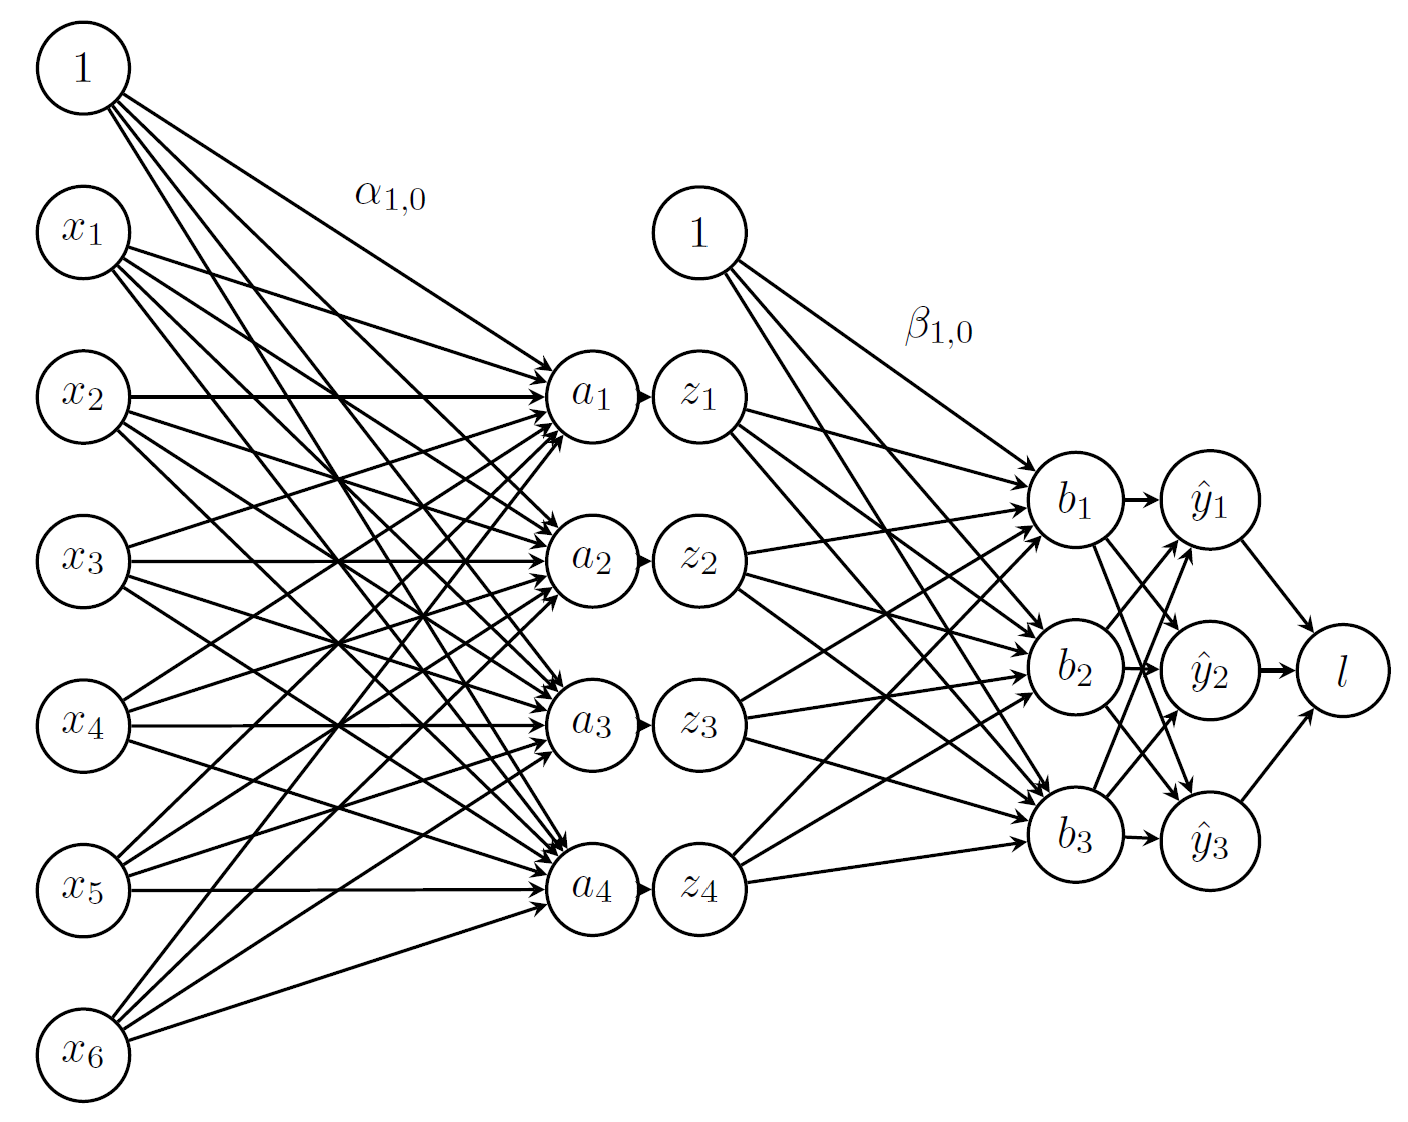
\includegraphics[height=9cm]{img/network.png}
        \caption{A One Hidden Layer Neural Network}
        \label{fig:oneHL}
    \end{figure}

\subsubsection*{\textcolor{purple}{Network Overview}}
Consider the neural network with one hidden layer shown in Figure \ref{fig:oneHL}. The input layer consists of 6 features $\xv = [x_1,...,x_6]^T$, the hidden layer has 4  nodes $\zv = [z_1,...,z_4]^T$, and the output layer is $\hat{\yv} = [\hat{y}_1, \hat{y}_2, \hat{y}_3]^T$ that sums to one over 3 classes. We also add a bias to the input, $x_0 = 1$ and the hidden layer $z_0 = 1$, both of which are fixed to $1$.


We adopt the following notation:
\begin{enumerate}
    \item Let \textcolor{magenta}{$\boldsymbol{\alpha}$} be the matrix of weights from the inputs to the hidden layer.
    \item Let \textcolor{magenta}{$\boldsymbol{\beta}$} be the matrix of weights from the hidden layer to the output layer.
    \item Let \textcolor{magenta}{$\alpha_{j,i}$} represent the weight going \textit{to} the node $z_j$ in the hidden layer \textit{from} the node $x_i$ in the input layer (e.g. $\alpha_{1,2}$ is the weight from $x_2$ to $z_1$)
    \item Let \textcolor{magenta}{$\boldsymbol{\beta}_{k,j}$} represent the weight going \textit{to} the node $y_k$ in the output layer \textit{from} the node $z_j$ in the hidden layer.
    \item We will use a \emph{sigmoid activation function (\textcolor{magenta}{$\sigma$})} for the hidden layer and a \emph{softmax} for the output layer. 
\end{enumerate}

\subsubsection*{\textcolor{purple}{Network Details}}
Equivalently, we define each of the following. 

The input:
\begin{align}
\xv=[x_1,x_2,x_3,x_4,x_5,x_6]^T
\end{align}

Linear combination at first (hidden) layer:
\begin{equation}
\label{eq:a_j}
a_j= \alpha_{j,0} + \sum_{i=1}^6 \alpha_{j,i}x_i,\quad j \in \{1,\ldots,4\}
\end{equation}

Activation at first (hidden) layer:
\begin{align}
\label{eq:z_j}
z_j &= \sigma(a_j) = \frac{1}{1+\exp(-a_j)},\quad  j \in \{1,\ldots,4\}
\end{align}

Linear combination at second (output) layer:
\begin{equation}
\label{eq:b_k}
b_k = \beta_{k,0} + \sum_{j=1}^4 \beta_{k,j}z_j,\quad  k \in \{1,\ldots,3\}
\end{equation}

Activation at second (output) layer:
\begin{equation}
\hat{y}_k = \frac{\exp(b_k)}{\sum\limits_{l=1}^3 \exp(b_l)},\quad  k \in \{1,\ldots,3\}
\end{equation}

Note that the linear combination equations can be written equivalently as the product of the weight matrix with the input vector. We can even fold in the bias term $\alpha_0$ by thinking of $x_0 = 1$, and fold in $\beta_0$ by thinking of $z_0 = 1$.

\subsubsection*{\textcolor{purple}{Loss}}

We will use cross entropy loss, $\ell(\hat{\yv},\yv)$. If $\yv$ represents our target (true) output, which will be a \textcolor{purple}{one-hot vector} representing the correct class, and $\hat{\yv}$ represents the output of the network, the loss is calculated as (note that the $\log$ terms are in base $e$):
\begin{equation}
\label{eq:cross_entropy_loss}
   \ell(\hat{\yv},\yv) = - \sum_{k=1}^3 y_k \log(\hat{y}_k)
\end{equation}
%%%%%%%%%%%%%%%%%%%%

\begin{enumerate}
\item \textbf{[6 pts]} In the following questions you will derive the matrix and vector forms of the previous equations which define our neural network. These are what you should hope to program in order to avoid excessive loops and large run times.\\
When working these out it is important to keep track of the vector and matrix dimensions in order for you to easily identify what is and isn't a valid multiplication. Suppose you are given a training example: $\xv^{(1)}=[x_1,x_2,x_3,x_4,x_5,x_6]^T$ with \textbf{label class 2}, so $\yv^{(1)}=[0,1,0]^T$. We initialize the network weights as:
\begin{center}
$$\boldsymbol{\alpha^*}=
    \begin{bmatrix}
    \alpha_{1,1} & \alpha_{1,2} & \alpha_{1,3} & \alpha_{1,4} & \alpha_{1,5} & \alpha_{1,6} \\
    \alpha_{2,1} & \alpha_{2,2} & \alpha_{2,3} & \alpha_{2,4} & \alpha_{2,5} & \alpha_{2,6} \\
    \alpha_{3,1} & \alpha_{3,2} & \alpha_{3,3} & \alpha_{3,4} & \alpha_{3,5} & \alpha_{3,6} \\
    \alpha_{4,1} & \alpha_{4,2} & \alpha_{4,3} & \alpha_{4,4} & \alpha_{4,5} & \alpha_{4,6}
    \end{bmatrix}$$
    
$$\boldsymbol{\beta^*}=
    \begin{bmatrix}
    \beta_{1,1} & \beta_{1,2} & \beta_{1,3} & \beta_{1,4} \\
    \beta_{2,1} & \beta_{2,2} & \beta_{2,3} & \beta_{2,4} \\
    \beta_{3,1} & \beta_{3,2} & \beta_{3,3} & \beta_{3,4}
    \end{bmatrix}
$$
\end{center}
    
We want to also consider the bias term and the weights on the bias terms (${\alpha}_{j,0}$ and ${\beta}_{k,0})$. To account for these we can add a new column to the beginning of our initial weight matrices. 

$$\boldsymbol{\alpha}=
    \begin{bmatrix}
    \textcolor{blue}{\alpha_{1,0}} & \alpha_{1,1} & \alpha_{1,2} & \alpha_{1,3} & \alpha_{1,4} & \alpha_{1,5} & \alpha_{1,6} \\
    \textcolor{blue}{\alpha_{2,0}} & \alpha_{2,1} & \alpha_{2,2} & \alpha_{2,3} & \alpha_{2,4} & \alpha_{2,5} & \alpha_{2,6} \\
    \textcolor{blue}{\alpha_{3,0}} & \alpha_{3,1} & \alpha_{3,2} & \alpha_{3,3} & \alpha_{3,4} & \alpha_{3,5} & \alpha_{3,6} \\
    \textcolor{blue}{\alpha_{4,0}} & \alpha_{4,1} & \alpha_{4,2} & \alpha_{4,3} & \alpha_{4,4} & \alpha_{4,5} & \alpha_{4,6}
    \end{bmatrix}$$
    
$$\boldsymbol{\beta}=
    \begin{bmatrix}
    \textcolor{blue}{\beta_{1,0}} & \beta_{1,1} & \beta_{1,2} & \beta_{1,3} & \beta_{1,4} \\
    \textcolor{blue}{\beta_{2,0}} & \beta_{2,1} & \beta_{2,2} & \beta_{2,3} & \beta_{2,4} \\
    \textcolor{blue}{\beta_{3,0}} & \beta_{3,1} & \beta_{3,2} & \beta_{3,3} & \beta_{3,4}
    \end{bmatrix}$$

    And we can set our first value of our input vectors to always be 1 ($x_0^{(i)} = 1$), so our input becomes: $$\xv^{(1)}=[\textcolor{blue}{1},x_1,x_2,x_3,x_4,x_5,x_6]^T$$
    
    
    \begin{enumerate}
        \item \textbf{[1 pt]} By examining the shapes of the initial weight matrices, how many neurons do we have in the first hidden layer of the neural network? (Not including the bias neuron)
        
        \begin{tcolorbox}[fit,height=1cm, width=2cm, blank, borderline={1pt}{-2pt}]
            %solution 
        \end{tcolorbox}
        
        
        
        
        \item \textbf{[1 pt]} How many output neurons will our neural network have?
        
        \begin{tcolorbox}[fit,height=1cm, width=2cm, blank, borderline={1pt}{-2pt}]
            %solution 
        \end{tcolorbox}
        

        
        
        
        
        \item \textbf{[1 pt]} What is the vector $\av$ whose elements are made up of the entries $a_j$ in equation (\ref{eq:a_j}). Write your answer in terms of $\alphav$ and $\xv^{(1)}$.
        
        
        \begin{tcolorbox}[fit,height=1cm, width=4cm, blank, borderline={1pt}{-2pt}]
            %solution 
        \end{tcolorbox}
        

        
        
        
        \item \textbf{[1 pt]} What is the vector $\zv$ whose elements are made up of the entries $z_j$ in equation (\ref{eq:z_j})? Write your answer in terms of $\av$.
        
        \begin{tcolorbox}[fit,height=1cm, width=4cm, blank, borderline={1pt}{-2pt}]
            %solution 
        \end{tcolorbox}
        
        
        \item \textbf{[1 pt]} \textbf{Select one:} We cannot take the matrix multiplication of our weights $\betav$ and our vector $\zv$ since they are not compatible shapes. Which of the following would allow us to take the matrix multiplication of $\betav$ and $\zv$ such that the entries of the vector $\bv = \betav\zv$ are equivalent to the values of $b_k$ in equation (\ref{eq:b_k})? 
        
        \begin{list}{}
        \item $\circle$ Remove the last column of $\betav$
        \item $\circle$ Remove the first row of $\zv$
        \item $\circle$ Append a value of 1 to be the first entry of $\zv$
        \item $\circle$ Append an additional column of 1's to be the first column of $\betav$ 
        \item $\circle$ Append a row of 1's to be the first row of $\betav$ 
        \item $\circle$ Take the transpose of $\betav$
        \end{list}

        \newpage
        
        \item \textbf{[1 pt]} What are the entries of the output vector $\hat{\yv}$? Your answer should be written in terms of $b_1,b_2,b_3$.
        
        \begin{tcolorbox}[fit,height=4cm, width=15cm, blank, borderline={1pt}{-2pt}]
            %solution 
        \end{tcolorbox}
        
        
    \end{enumerate} 

\item \textbf{[7 pts]} We will now derive the matrix and vector forms for the backpropagation algorithm.

$$\frac{d\ell}{d\alphav} = 
    \begin{bmatrix}
        \adj{\alpha_{10}} & \adj{\alpha_{11}} & \dots  & \adj{\alpha_{1M}} \\
        \adj{\alpha_{20}} & \adj{\alpha_{21}} & \dots  & \adj{\alpha_{2M}} \\
        \vdots      & \vdots      & \ddots & \vdots \\
        \adj{\alpha_{D0}} & \adj{\alpha_{D1}} & \dots  & \adj{\alpha_{DM}}
    \end{bmatrix}$$




Recall that $\ell$ is our loss function defined in equation (\ref{eq:cross_entropy_loss})
    
    \begin{enumerate}
        \item \textbf{[1 pt]} The derivative of the softmax function with respect to $b_k$ is as follows:
        $$\frac{d\hat{y}_l}{db_k} = \hat{y}_l(\Ib[k=l]-\hat{y}_k)$$ 
        where $\Ib[k=l]$ is an indicator function such that if $k=l$ then it it returns value 1 and 0 otherwise. 
        Using this, write the derivative $\frac{d\ell}{db_k}$ in a smart way such that you do not need this indicator function. Write your solutions in terms of $\hat{y}_k,y_k$.
        
        
        \begin{tcolorbox}[fit,height=2cm, width=12cm, blank, borderline={1pt}{-2pt}]
            %solution 
        \end{tcolorbox}
        
        
        \item \textbf{[1 pt]} What are the elements of the vector $\frac{d\ell}{db}$? (Recall that  $\yv^{(1)}=[0,1,0]^T$)
        
        
        \begin{tcolorbox}[fit,height=1cm, width=6cm, blank, borderline={1pt}{-2pt}]
            %solution 
        \end{tcolorbox}
        
        
        \item \textbf{[1 pt]} What is the derivative $\frac{d\ell}{d\beta}$? Your answer should be in terms of $\frac{d\ell}{d\bv}$ and $\zv$.
        
        
        \begin{tcolorbox}[fit,height=3cm, width=12cm, blank, borderline={1pt}{-2pt}]
            %solution 
        \end{tcolorbox}
        
        
        
        \item \textbf{[1 pt]} Explain in one short sentence why must we go back to using the matrix $\betav^*$ (The matrix $\betav$ without the first column of bias weights) when calculating the matrix $\frac{d\ell}{d\alpha}$?
        
        
        \begin{tcolorbox}[fit,height=1cm, width=15cm, blank, borderline={1pt}{-2pt}]
            %solution 
        \end{tcolorbox}
        
        
        \item \textbf{[1 pt]} What is the derivative $\frac{d\ell}{d\zv}$? Your answer should be in terms of $\frac{d\ell}{d\bv}$ and $\betav^*$
        
        
        \begin{tcolorbox}[fit,height=3cm, width=12cm, blank, borderline={1pt}{-2pt}]
            %solution 
        \end{tcolorbox}
        
    
        \item \textbf{[1 pt]} What is the derivative $\frac{d\ell}{d\av}$ in terms of $\frac{d\ell}{d\zv}$ and $\zv$
        
        
        \begin{tcolorbox}[fit,height=3cm, width=12cm, blank, borderline={1pt}{-2pt}]
            %solution 
        \end{tcolorbox}
        
        
        \item \textbf{[1 pt]} What is the matrix $\frac{d\ell}{d\alpha}$? Your answer should be in terms of $\frac{d\ell}{d\av}$ and $x^{(1)}$.
        
        
        \begin{tcolorbox}[fit,height=3cm, width=12cm, blank, borderline={1pt}{-2pt}]
            %solution 
        \end{tcolorbox}

\end{enumerate}



%%%%%%%%%%%%%%%%%%%%%%%%
\subsubsection*{\textcolor{purple}{Prediction}}
When doing prediction, we will predict the \textcolor{purple}{$\argmax$} of the output layer. For example, if $\hat{\yv}$ is such that $\hat{y}_1=0.3,~ \hat{y}_2=0.2,~ \hat{y}_3=0.5$ we would predict class 3 for the input $\xv$. If the true class from the training data $\xv$ was $2$ we would have a \textcolor{purple}{one-hot vector} $\yv$ with values $y_1=0$,~ $y_2=1$,~ $y_3=0$.
    
\item \textcolor{black}{\textbf{[8 pts]}}
     We initialize the weights as:
\begin{center}
$$\boldsymbol{\alpha^*}=
    \begin{bmatrix}
    2 & 1 & -1 & -1 & 0 & -2 \\
    0 & 1 & 0 & -1 & 1 & 3 \\
    -1 & 2 & 1 & 3 & 1 & -1 \\
    1 & 3 & 4 & 2 & -1 & 2
    \end{bmatrix}$$
$$\boldsymbol{\beta^*}=
    \begin{bmatrix}
    2 & -2 & 2 & 1 \\
    3 & -1 & 1 & 2 \\
    0 & -1 & 0 & 1
    \end{bmatrix}
$$
\end{center}
    
And weights on the bias terms (${\alpha}_{j,0}$ and ${\beta}_{j,0})$ are initialized to 1.
    
    You are given a training example $\xv^{(1)}=[1,0,1,0,1,0]^T$ with label class 2, so $\yv^{(1)}=[0,1,0]^T$. Using the initial weights, run the feed forward of the network over this training example (without rounding during the calculation) and then answer the following questions. 
    
    \begin{enumerate}
        \item \textbf{[1 pt]} What is the value of $a_1$?
        
        \begin{tcolorbox}[fit,height=1cm, width=2cm, blank, borderline={1pt}{-2pt}]
            %solution 
        \end{tcolorbox}
        
        
        \item \textbf{[1 pt]} What is the value of $z_1$?
        
        \begin{tcolorbox}[fit,height=1cm, width=2cm, blank, borderline={1pt}{-2pt}]
         %solution 
        \end{tcolorbox}

        
        \item \textbf{[1 pt]} What is the value of $a_3$?
        
        \begin{tcolorbox}[fit,height=1cm, width=2cm, blank, borderline={1pt}{-2pt}]
        %solution 
        \end{tcolorbox}
        
        
        \item \textbf{[1 pt]} What is the value of $z_3$?
        
        \begin{tcolorbox}[fit,height=1cm, width=2cm, blank, borderline={1pt}{-2pt}]
            %solution 
        \end{tcolorbox}
        
        
        \item \textbf{[1 pt]} What is the value of $b_2$?
        
        \begin{tcolorbox}[fit,height=1cm, width=2cm, blank, borderline={1pt}{-2pt}]
            %solution 
        \end{tcolorbox}
        
        
        \item \textbf{[1 pt]} What is the value of $\hat{y}_2$?
        
        \begin{tcolorbox}[fit,height=1cm, width=2cm, blank, borderline={1pt}{-2pt}]
            %solution 
        \end{tcolorbox}
        
        
        \item \textbf{[1 pt]} Which class value we would predict on this training example?
        
        \begin{tcolorbox}[fit,height=1cm, width=2cm, blank, borderline={1pt}{-2pt}]
            %solution 
        \end{tcolorbox}
        

        \item \textbf{[1 pt]} What is the value of the total loss on this training example?
        
        \begin{tcolorbox}[fit,height=1cm, width=2cm, blank, borderline={1pt}{-2pt}]
            %solution 
        \end{tcolorbox}
        
        
    \end{enumerate}
    
\item \textcolor{black}{\textbf{[3 pts]}} Now use the results of the previous question to run backpropagation over the network and update the weights. Use the learning rate $\eta=1$. 
    
    Do your backpropagation calculations without any rounding then answer the following questions: (in your final responses round to four decimal places)
    
     \begin{enumerate}
        \item \textbf{[1 pt]} What is the updated value of ${\beta}_{2,1}$?
        
        \begin{tcolorbox}[fit,height=1cm, width=2cm, blank, borderline={1pt}{-2pt}]
            %solution 
        \end{tcolorbox}
        
        
        \item \textbf{[1 pt]} What is the updated weight of the hidden layer bias term applied to $y_1$ (i.e. ${\beta}_{1,0}$)?
        
        \begin{tcolorbox}[fit,height=1cm, width=2cm, blank, borderline={1pt}{-2pt}]
            %solution 
        \end{tcolorbox}
        
        \item \textbf{[1 pt]} What is the updated value of ${\alpha}_{3,4}$?
        
        \begin{tcolorbox}[fit,height=1cm, width=2cm, blank, borderline={1pt}{-2pt}]
            %solution 
        \end{tcolorbox}
        
    \end{enumerate}

    \newpage

\item \textcolor{black}{\textbf{[5 pts]}} Let us now introduce regularization into our neural network. For this question, we will incorporate L2 regularization into our loss function $\ell(\hat{\yv},\yv)$, with the parameter $\lambda$ controlling the weight given to the regularization term. 
\begin{enumerate}
    \item \textbf{[1 pt]} Write the expression for the regularized loss function of our network after adding L2 regularization (\textbf{Hint:} Remember that bias terms should not be regularized!) 
    \begin{tcolorbox}[fit,height=3cm, width=15cm, blank, borderline={1pt}{-2pt}]
            %solution 
    \end{tcolorbox}
    
    \item \textbf{[1 pts]} Compute the regularized loss for training example $\xv^{(1)}$ (assume $\lambda$ = 0.01 and use the weights before backpropagation)
    \begin{tcolorbox}[fit,height=1cm, width=2cm, blank, borderline={1pt}{-2pt}]
            %solution 
    \end{tcolorbox}   
    
     \item \textbf{[1 pts]} For a network which uses the regularized loss function, write the gradient update equation for $\alpha_{j,i}$ . You may use $\frac{\partial \ell(\hat{\yv},\yv)}{\partial \alpha_{j,i}}$ to denote the gradient update w.r.t non-regularized loss and $\eta$ to denote the learning rate.
    \begin{tcolorbox}[fit,height=3cm, width=15cm, blank, borderline={1pt}{-2pt}]
            %solution 
    \end{tcolorbox}

    \item \textbf{[2 pts]} Based on your observations from previous questions, \textbf{select all statements which are true}:
    \begin{list}{}
    \item $\square$ The non-regularized loss is always higher than the regularized loss 
    \item $\square$ As weights become larger, the regularized loss increases faster than non-regularized loss
    \item $\square$ On adding regularization to the loss function, gradient updates for the network become larger
    \item $\square$ When using large initial weights, weight values decrease more rapidly for a network which uses regularized loss 
    \item $\square$ None of the above
    \end{list}
    
\end{enumerate}
\end{enumerate}

\clearpage
\section{{Neural Net Programming [40 pts]}}
\label{sec:code}

\begin{figure}[H]
    \centering
    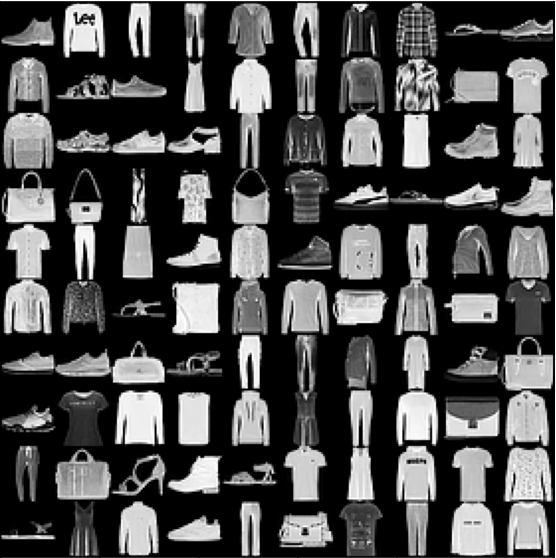
\includegraphics[scale=0.8]{img/tiled_mnist.png}
    \caption{Random Images of Each of 10 classes in Fashion-MNIST}
    \label{fig:grid}
\end{figure}

Your goal in this assignment is to label images of fashion articles by implementing a neural network from scratch. You will implement all of the functions needed to initialize, train, evaluate, and make predictions with the network. \textbf{Important: You must use PyTorch to complete this assignment. However, you are not allowed to directly use builtin PyTorch modules (e.g., nn.Linear, nn.Sigmoid, nn.Softmax, etc...) for the module implementations. Same for the corresponding forward() and backward() function implementations.)}

The Fashion-MNIST dataset is comprised of 70,000 images of fashion articles and their respective labels. There are 60,000 training images and 10,000 test images, all of which are 28 pixels by 28 pixels. The images belong to the following 10 categories -- [T-shirt, Trouser, Pullover, Dress, Coat, Sandal, Shirt, Sneaker, Bag, Ankle boot].


\paragraph{Dataset format} In the file \texttt{nn\_implementation\_code/base\_experiment.py} there are lines for downloading the dataset and converting it to the \texttt{torch.utils.data.Dataset} format. More information about \texttt{torch.utils.data.Dataset} and \texttt{torch.utils.data.Dataloader} can be found in \href{https://pytorch.org/tutorials/beginner/basics/data_tutorial.html}{this tutorial}; you may use these classes to operate with data and batches.

\textbf{Note:} We strongly encourage you to do the written part of this homework before the programming, as it will help you gain familiarity with the calculations you will have to code up in the programming section. We suggest that for each of these problems, you write out the equation required to calculate each value in terms of the variables we created ($a_j, z_j, b_k$, etc.) before you calculate the numerical value.


\textbf{Note:} For all questions which require numerical answers, round up your final answers to four decimal places. You will be submitting the files: \texttt{base\_experiment.py}, \texttt{custom\_functions.py}, and \texttt{custom\_modules.py} on Gradescope.

\newpage

\subsection*{\textcolor{blue}{Model Definition}}
\subsubsection*{\textcolor{purple}{Preliminaries}}
In this section, you will implement a single-hidden-layer neural network with a sigmoid activation function for the hidden layer, and a softmax on the output layer. For this particular problem, the input vectors $\xv$ are of length $M = 28\times 28$, the hidden layer $\zv$ consist of $D$ hidden units, and the output layer $\hat{\yv}$ represents a probability distribution over the $K = 10$ classes. In other words, each element $\hat{y}_k$ of the output vector $\hat{\yv}$ represents the probability of $\xv$ belonging to the class $k$. 

Following the notation from the written section we have:
\begin{itemize}
    \item For the output layer:
    \begin{gather*}
         \hat{y}_k = \frac{\exp(b_k)}{\sum_{l=1}^K \exp(b_l)},\quad k\in\{1,\dots,K\},\quad (\text{softmax activation})\\[3mm]
         b_k =  \beta_{k,0} + \sum_{j=1}^D \beta_{kj} z_j,\quad k\in\{1,\dots,K\},\quad (\text{pre-activation})
    \end{gather*}    
    \item For the hidden layer:
    \begin{gather*}
        z_j = \frac{1}{1+\exp(-a_j)},\quad j\in\{1,\dots,D\},\quad (\sigma-\text{activation})\\[3mm]
        a_j = \alpha_{j,0} + \sum_{i=1}^M \alpha_{ji} x_i,\quad j\in\{1,\dots,D\},\quad (\text{pre-activation})
    \end{gather*}        
\end{itemize}


It is possible to compactly express this model by assuming that $x_0=1$ is a bias feature on the input and that $z_0=1$ is also fixed. In this way, we have two parameter matrices $\alphav \in \Rb^{D \times (M+1)}$ and $\betav \in \Rb^{K \times (D+1)}$. The extra $0$th column of each matrix (i.e. $\alphav_{\cdot,0}$ and $\betav_{\cdot,0}$) hold the bias parameters. With these considerations we have,

\begin{gather*}
\hat{y}_k = \frac{\exp(b_k)}{\sum_{l=1}^K \exp(b_l)},\quad k\in\{1,\dots,K\}
\\[3mm]
b_k =  \sum_{j=0}^D \beta_{kj} z_j,\quad k\in\{1,\dots,K\}
\\[3mm]
z_j = \frac{1}{1+\exp(-a_j)},\quad j\in\{1,\dots,D\}
\\[3mm]
a_j = \sum_{i=0}^M \alpha_{ji} x_i,\quad j\in\{1,\dots,D\}
\end{gather*}


\newpage

\subsubsection*{\textcolor{purple}{Objective function}}
Since the output corresponds to a probabilistic distribution over the $K$ classes, the objective (cost) function we will use for training our neural network is the \textcolor{magenta}{average cross entropy},
\begin{gather}
\label{eq:celoss}
J(\alphav, \betav)= - \frac{1}{N} \sum_{n=1}^N \sum_{k=1}^{K} y_k^{(n)} \log (\hat{y}^{(n)}_k)
\end{gather}
over the training dataset,
\begin{gather*}
\Dc = \{ (\xv^{(n)}, \yv^{(n)})\}, \quad\text{for $n\in\{1,\ldots N\}$} 
\end{gather*}


In Equation~\eqref{eq:celoss}, $\textcolor{magenta}{J}$ is a function of the model parameters $\alphav$ and $\betav$ because $\hat{y}^{(n)}_k$ is implicitly a function of $\xv^{(n)}$, $\alphav$, and $\betav$ since it is the output of the neural network applied to $\xv^{(n)}$. As before, $\hat{y}^{(n)}_k$ and $y_k^{(n)}$ present the $k$-th component of $\hat{\yv}^{(n)}$ and $\yv^{(n)}$ respectively.


To train the network, you should optimize this objective function using \textcolor{magenta}{stochastic gradient descent (SGD)}, where the gradient of the parameters for each training example is computed via \textcolor{magenta}{backpropagation}, though typically you should shuffle your data during SGD you are \textbf{not} to do so here, and instead you are to train through the dataset in the order it is given.

\subsection*{\textcolor{blue}{Implementation}}
\label{sec:model}

To proceed, you are provided with the following guide. This is recommended but absolutely not required.

\subsubsection*{\textcolor{purple}{Defining layers}}

Just to recap, your network architecture should look like the following:
 \texttt{Linear}$\rightarrow$ \texttt{Sigmoid} $\rightarrow$ \texttt{Linear} $\rightarrow$ \texttt{Softmax}.
 The size of the input is 784. The first linear layer can have 785 nodes to include bias term. The final (output) layer should have 10 nodes (one corresponding to each integer from 0 - 9). The hidden layer will have D = 256 nodes (excluding bias term).


\textbf{Again, you are not allowed to directly use built-in PyTorch modules (e.g.,
nn.Linear, nn.Sigmoid, nn.Softmax, etc...) for the module implementations}. Instead,
you should complete the methods defined for you all in \texttt{custom\_functions.py} to
implement your own versions of these layers.
    
\textbf{Be aware of computing issues!} $\log(x)$ is problematic when $x\rightarrow0$. Similarly $exp(x)$ may overflow
when it is huge. Think of using $\log$ to avoid some exponential calculations and dividing both numerator and denominator by a large value to avoid overflowing:
$$\frac{e^{x_i}}{\sum e^{x_j}} = \frac{e^{x_i-b}}{\sum e^{x_j-b}}$$


\subsubsection*{\textcolor{purple}{Pseudo-code for Training Loop}}
\begin{lstlisting}
For epoch in epochs:
	for x, y in train_x, train_y:
		Pass x through all the forward layers and get the loss
		Pass the output though all the backward layers
		Update weights and biases
	compute the average training loss for the epoch
	compute test loss
	compute test accuracy
\end{lstlisting}

You can follow the steps mentioned above or approach it any other way. 

\subsubsection*{\textcolor{purple}{Important Tips}}
\begin{itemize}
    \item The training loss you report, should not be aggregated throughout an epoch, rather you should compute the loss on the whole training set at the end of each epoch.
   
    \item When performing mini-batch gradient descent, you should take the mean of the loss within a batch before applying the update.
    \item Do NOT shuffle the training or test data, otherwise the answers won't match. 
\end{itemize}

\subsection*{\textcolor{blue}{Programming Submission}}
\textbf{NOTE: Initial weights and biases are provided in the file \texttt{weights.pt}. Use the following hyper-parameters:
\begin{itemize}
    \item Learning rate = 0.01
    \item Width of hidden layer = 256 (excluding bias)
\end{itemize}}
We have provided the outputs of first five nodes of each layer and the updated weights for the first data point in the first epoch in the folder \texttt{check}, trained with batch size 1. Use these to verify your implementation.


\begin{enumerate}

    \item \textbf{[15 pts]} Firstly, pass the programming tests on Gradescope. Make sure that your implementation gets full points before moving on to the experiments below.

    
    \item \textbf{[2 pts]} Train the model on batches of data i.e. a mini-batch gradient descent. Run the model for 50 epochs with a batch size of 5, and report the average final training loss and the test accuracy. Report numbers till 4 places of decimal.

    
    \begin{tcolorbox}[fit,height=1cm, width=5cm, blank, borderline={1pt}{-2pt}]
    Training Loss: %solution 
    \end{tcolorbox}
    \begin{tcolorbox}[fit,height=1cm, width=5cm, blank, borderline={1pt}{-2pt}]
    Test Accuracy: %solution 
    \end{tcolorbox}
    
    \clearpage
    \item \textbf{[4 pts]} For the model trained for 50 epochs, display the confusion matrix for both the training and test sets. In the plot, you should have \emph{true labels} on the y-axis and \emph{predicted labels} on the x-axis. For example, the second entry in the fourth row should show the count for the number of times class 3 was wrongly predicted as 1.
    
    \begin{tcolorbox}[fit,height=8cm, width=0.95\textwidth, blank, borderline={1pt}{-2pt}]
            %solution 
    \end{tcolorbox}
    
    
    \item \textbf{[2 pts]} For each class, display the first data point in the test dataset that was wrongly classified.

    \begin{tcolorbox}[fit,height=3cm, width=0.95\textwidth, blank, borderline={1pt}{-2pt}]
            %solution 
    \end{tcolorbox}
    
    \clearpage
    \item \textbf{[8 pts]} Now we will experiment with different batch sizes. For each batch size in [10, 50, 100], run your model for 50 epochs. Plot two graphs of epoch vs loss, one each for training and test loss, which have the epoch number on the x-axis and the loss value on the y-axis.  Please make sure your graphs are properly labeled and include a legend showing the color for each batch size.
    
    \begin{tcolorbox}[fit,height=8cm, width=0.95\textwidth, blank, borderline={1pt}{-2pt}]
    %solution 
    \end{tcolorbox}

    
    \item \textbf{[2 pts]} Based on the plots in the previous part, what do you observe about the effect of increasing batch sizes? How does this relate to the learning rate? (Explain in 1-2 lines)

    \begin{tcolorbox}[fit,height=2cm, width=0.95\textwidth, blank, borderline={1pt}{-2pt}]
            %solution 
    \end{tcolorbox}
        
    
    \item \textbf{[2 pts]} Based on the plots in the part 5 of the programming question, what do you think is the best next step given the trends of different batch sizes? (Explain in 1-2 lines)

    \begin{tcolorbox}[fit,height=2cm, width=0.95\textwidth, blank, borderline={1pt}{-2pt}]
            %solution 
    \end{tcolorbox}
        
    \clearpage
    \item  \textbf{[5 pts]} Now we want to give you a chance to experiment with the model by exploring the hyper-parameters of a neural network. Produce a pair of plots similar to that of the one requested in the batch size experiment, by varying a different hyperparameter in the network. Experiment with at least 3 different values for the hyperparameter that you decide to modify. For your experiment, you must,

    \begin{enumerate}[label=(\alph*)]
        \item describe the hyperparameter you varied
        \item list the values you set the hyperparameter to
        \item detail the setting of all the other hyperparameters, and
        \item analyze your results in terms of the hyperparameter that you varied.
    \end{enumerate}
    
    For your reference here are some hyperparameters which you can change:
    \begin{itemize}
        \item Learning Rate
        \item Width of Hidden Layer
        \item Different weight initialization
    \end{itemize}

     You may choose any reasonable batch size and number of epochs for this question, just make sure to specify all design decisions you make. This question is for learning so feel free to experiment with whatever hyperparameter you wish to, as long you can provide a reasonable explanation for the observed behavior in the graphs.
    
    \begin{tcolorbox}[fit,height=10cm, width=0.95\textwidth, blank, borderline={1pt}{-2pt}]
    Experiment %solution 
    \end{tcolorbox}
\end{enumerate}

\clearpage
\section{Collaboration Questions}

\begin{enumerate}
    \item 
    \begin{enumerate}
        \item Did you receive any help whatsoever from anyone in solving this assignment? 

        \item If you answered `yes', give full details (e.g. “Jane Doe explained to me what is asked in Question 3.4”)\\
        
        \begin{tcolorbox}[fit,height=4cm, width=15cm, blank, borderline={1pt}{-2pt},nobeforeafter]

        
        \end{tcolorbox}
        
    \end{enumerate}
    
    
    \item 
    \begin{enumerate}
        \item Did you give any help whatsoever to anyone in solving this assignment? 

        
        \item If you answered `yes', give full details (e.g. “I pointed Joe Smith to section 2.3 since he didn’t know how to proceed with Question 2”)\\
        
        \begin{tcolorbox}[fit,height=4cm, width=15cm, blank, borderline={1pt}{-2pt},nobeforeafter]
        
        
        \end{tcolorbox}
        
    \end{enumerate}
    
    \item 
    \begin{enumerate}
        \item Did you find or come across code that implements any part of this assignment?

        
        \item If you answered `yes', give full details (book \& page, URL \& location within the page, etc.).\\
        
        \begin{tcolorbox}[fit,height=4cm, width=15cm, blank, borderline={1pt}{-2pt},nobeforeafter]
        
        
        \end{tcolorbox}
        
    \end{enumerate}
\end{enumerate}

\end{document}
